\documentclass[12pt]{article}

\usepackage{amsmath}
\usepackage{amsfonts}
\usepackage{amssymb}
\usepackage{graphicx}
\usepackage[center]{caption}
\usepackage{mathtools}
\usepackage{lipsum}
\usepackage{stackengine}
\usepackage{fancyhdr}
\usepackage{caption}
\usepackage{tikz}
\usetikzlibrary{shapes.geometric, arrows}
\usepackage{float}
\usepackage[a4paper,left=1in,right=1in,top=1in,bottom=1in,footskip=.25in]{geometry}
\usepackage{etoolbox}
\usepackage[nottoc]{tocbibind}
\usepackage{tabu}
\usepackage{enumitem,kantlipsum}
\usepackage{verbatim}
\begin{document}
	\begin{titlepage}
		\centering
		
		\begin{figure}
			\begin{center}
				
\includegraphics[scale=.2]{tubaf.pdf}  
			\end{center}
			
		\end{figure}
		
		
		
		%\includegraphics[width=0.15\textwidth]{download}\par\vspace{1cm}
		{\scshape\LARGE Technische Universit\"at Bergakademie Freiberg \par}
		\vspace{1cm}
		{\scshape\Large PERSONAL PROGRAMMING PROJECT\par}
		\vspace{1.5cm}
		{\huge\bfseries Implementation of Iso-geometric Analysis (IGA) for Piezoelectric Material \par}
		\vspace{2cm}
		{\scshape\Large Vikas Diddige\par}
		{\scshape\Large 64041\par}
		\vfill
		{\normalsize\ Supervised by\par}
		
		Dr.~ \textsc{Sergii Kozinov}
		
		\vfill
		
		% Bottom of the page
		{\large \today\par}
	\end{titlepage}
	
	\clearpage
	\textbf{\LARGE Abstract}\\ \newline
	\newline
	
	
	\newpage
	\clearpage
	\tableofcontents
	\clearpage
	
\section{Introduction}
Among all the numerical methods Finite Element Methods (FEM) are more popularly used to find approximate solutions of partial differential equations. FEM approximates the Computer Aided Drawing (CAD) geometry by discretizing it into smaller geometries called elements. Such geometrical approximations may create numerical errors and seriously effect the accuracy of the solution.
Isogeometric analysis (IGA) is a technique to generate geometry using CAD concept of Non Uniform Rational B-Splines (NURBS) and analyse using its basis functions. !The pioneers of this technique are Tom Hughes and his group at The University of Texas at Austin!.


\subsection{Advantages of IGA over FEA}
\begin{description}[leftmargin=*]
	\item[$\bullet$]   The exact representation of the geometry for analysis rules out the possibility of geometrical approximations.
	\item[$\bullet$]   A huge amount of time involved in finite element modelling can be avoided.
\end{description}

\section{B-Splines } \label{BSplines}
In this section a brief description of B-Splines is discussed since NURBS is an extended version of B-Splines. A B-Spline basis function is defined by its order and knot vectors. A B-spline basis function along with control points defines a B-Spline curve.
\subsection{Order }
For a point on a B-Spline curve the order of the basis function speaks about the number of nearby control points influence the given point. The degree $p$ of the basis function is one less than the order of the curve.

\subsection{Knot vector }
A knot vector is an array with an ascending order of parameter values written as $\Xi = \{ \xi_0,\xi_1,\xi_2.....,\xi_{n+p}\}$.
!The knot vector is a sequence of parameter values that determines where and how the control points affect the NURBS curve. The number of knots is always equal to the number of control points plus curve degree plus one (i.e. number of control points plus curve order). The knot vector divides the parametric space in the intervals mentioned before, usually referred to as knot spans. Each time the parameter value enters a new knot span, a new control point becomes active, while an old control point is discarded. It follows that the values in the knot vector should be in nondecreasing order, so (0, 0, 1, 2, 3, 3) is valid while (0, 0, 2, 1, 3, 3) is not.(WIKI)!

\subsection{Control points }
!The control points determine the shape of the curve.[8] Typically, each point of the curve is computed by taking a weighted sum of a number of control points. The weight of each point varies according to the governing parameter. For a curve of degree d, the weight of any control point is only nonzero in d+1 intervals of the parameter space. Within those intervals, the weight changes according to a polynomial function (basis functions) of degree d. At the boundaries of the intervals, the basis functions go smoothly to zero, the smoothness being determined by the degree of the polynomial.(WIKI)! The total number of control points is given by $n_{cp}(\xi)$ = total number of knots in $[\Xi] - (p+1)$. *****



\subsection{B-Spline basis functions }

For a given Knot vector $\Xi$, the B-spline basis function for polynomial degree $\geq 1$ is defined by a recursive function

\begin{equation}
N_{i,p}(\xi) = \frac{\xi-\xi_{i}}{\xi_{i+p}-\xi_{i}} N_{i,p-1}(\xi) + 
\frac{\xi_{i+p+1}-\xi}{\xi_{i+p+1}-\xi_{i+1}} N_{i+1,p-1}(\xi)
\end{equation}

\noindent
with
\begin{equation}
 N_{i,0}(\xi) = 
\begin{cases*}
1 \quad& if $  \xi_{i} \leq \xi<\xi_{i+1} $ \\
0 &  $ otherwise $ \\
\end{cases*}
\end{equation}

\subsubsection{Properties }
\begin{enumerate}
\item $ N_{i,0}(\xi)$ is a step wise function with a value 1 over the half open interval $ \xi \in [\xi_{i}  \leq \xi<\xi_{i+1}) $ and zero on the rest.
\item Basis functions sum upto to unity $\sum_{i=0}^{n} N_{i,p}(\xi) =1$
\item Basis functions are non-negative $ N_{i,p}(\xi) \geq 0$ over the entire
 domain
\item********** Write more*********** 
\end{enumerate}

\subsubsection{Derivatives }
The first derivative of a B-Spline basis function with its variable $\xi$ is given by

\begin{equation}
\frac{d}{d\xi}N_{i,p}(\xi) = \frac{p}{\xi_{i+p}-\xi_{i}} N_{i,p-1}(\xi) -
\frac{p}{\xi_{i+p+1}-\xi_{i+1}} N_{i+1,p-1}(\xi)
\end{equation}

\noindent
Higher order derivatives are not necessary for IGA formulation.

\subsection{B-Spline curves}

A $pth-degree$ B-Spline curve with a set of control points $P_i$ is given by
\begin{equation}
C(\xi) = \sum_{i=0}^{n} N_{i,p}(\xi) P_i \qquad \xi_0 \leq \xi \leq \xi_{n+p}
\end{equation}

\noindent
defined on the knot vector $\Xi = \{ \xi_0,\xi_1,\xi_2.....,\xi_{n+p}\}$

\subsection{B-Spline surfaces}
A B-Spline surface $S(\xi,\eta)$ is built by tensor product between B-Spline curves along each parametric direction ($\xi,\eta$). It requires knot vectors ($\Xi = \{ \xi_0,\xi_1,\xi_2.....,\xi_{n+p}\}$,$H = \{\eta_0,\eta_1,\eta_2.....,\eta_{m+q}\}$) along each parametric direction and control net $P_{i,j}$


\begin{equation} \label{BSplineSurface}
S(\xi,\eta) = \sum_{i=0}^{n}\sum_{j=0}^{m} N_{i,p}(\xi) N_{j,q}(\eta) P_{i,j}
\end{equation}

\noindent
where
p,q are the degrees of the B-Spline basis functions along $\xi,\eta$ respectively and n,m are number of control points along $\xi,\eta$ respectively.
\noindent
Eq. (\ref{BSplineSurface}) can be compactly written as

\begin{equation} \label{BSplineSurface}
S(\xi,\eta) = \sum_{i=0}^{n}\sum_{j=0}^{m} N_{i,j}^{p,q}(\xi,\eta) P_{i,j}
\end{equation}

\subsubsection{Derivatives}

The partial derivatives of bivariate B-Spline basis functions w.r.t parametric co-ordinates is given as

\begin{equation} 
\frac{\partial N_{i,j}^{p,q}(\xi,\eta)}{\partial \xi} = \frac{d}{d\xi} \bigg(N_{i,p}(\xi)\bigg)N_{j,q}(\eta) 
\qquad
\frac{\partial N_{i,j}^{p,q}(\xi,\eta)}{\partial \eta} = \frac{d}{d\eta} \bigg(N_{j,q}(\eta)\bigg)N_{i,p}(\xi)
\end{equation}















\section{Non Uniform Rational B-Splines } \label{NURBS}
NURBS are very often used in computer-aided design(CAD), manufacturing (CAM) and engineering (CAE) due to its flexibility to represent complex geometries. NURBS curves and surfaces are considered as the generalization of B-Spline and Bezier curves and surfaces. A NURBS basis function is defined by its order and knot vector.

\subsection{NURBS basis functions}
NURBS basis functions $R_{i,p}(\xi)$ are defined as
\begin{equation}
R_{i,p}(\xi) = \frac{N_{i,p}(\xi)w_{i}}{\sum_{i=0}^{n}N_{i,p}(\xi)w_{i}}
\end{equation}

\noindent
where $N_{i,p}(\xi)$ is the $i$th B-Spline basis function with order p and $w_{i}$ denotes weight of the $i$th control point ($P_i$). ***** Explain weights with help of an example****. When $w_{i} = constant \quad \forall i$ the NURBS basis function reduces to B-Spline basis function.
\subsubsection{Derivatives}
The first derivative of a NURBS basis function with its variable $\xi$ is given by

\begin{equation}
\frac{d }{d \xi} R_{i,p}(\xi) = \frac{N^{'}_{i,p}(\xi)  W(\xi) - N_{i,p}(\xi)  W^{'}(\xi)}{W^{2}(\xi)}w_{i}
\end{equation}
\noindent
where
$N^{'}_{i,p}(\xi) = \frac{d }{d \xi} N_{i,p}(\xi)$  \\
\\
\noindent
and $W^{'}(\xi) =  \sum_{i=0}^{n}N^{'}_{i,p}(\xi) w_i$


\subsection{NURBS Curves }
The $p^{th}$ degree NURBS curve is given by

\begin{equation}
C(\xi) = \frac{\sum_{i=0}^{n}N_{i,p}(\xi)w_{i}P_{i}}{\sum_{i=0}^{n}N_{i,p}(\xi)w_{i}}
\qquad \xi_0 \leq \xi \leq \xi_{n+p}
\end{equation}
in short form
\begin{equation}
C(\xi) = \sum_{i=0}^{n}R_{i,p}(\xi)P_{i}
\end{equation}
refer NURBS book and write more info
\subsection{NURBS Surfaces and solids }
NURBS Surfaces and solids are generated by the tensor product between NURBS curve basis functions.
\begin{enumerate}[leftmargin=*]
	\item NURBS Surfaces: \\
	A NURBS surface with degree $p$ in $\xi$ direction and degree $q$ in $\eta$ direction is defined as
	\begin{equation}
	S(\xi,\eta) = \sum_{i=0}^{n}\sum_{j=0}^{m} R_{i,j}^{p,q}(\xi,\eta)  P_{i,j}
	\end{equation}
	where the bivariate NURBS basis functions are given by
	\begin{equation}
	R_{i,j}^{p,q}(\xi,\eta)  = \frac{N_{i,p}(\xi)N_{j,q}(\eta)w_{i,j}}{\sum_{i=0}^{n}\sum_{j=0}^{m}N_{i,p}(\xi)N_{j,q}(\eta)w_{i,j}}
	\end{equation}
	\item NURBS Solids: \\
	A NURBS solid with degree $p,q,k$ in $\xi$, $\eta$, $\zeta$ directions respectively is defined as
	\begin{equation}
	S(\xi,\eta,\zeta) = \sum_{i=0}^{n}\sum_{j=0}^{m}\sum_{k=0}^{l} R_{i,j,k}^{p,q,r}(\xi,\eta,\zeta)  P_{i,j,k}
	\end{equation}
	where the $R_{i,j,k}^{p,q,r}(\xi,\eta,\zeta)$ is given by
	\begin{equation}
	R_{i,j,k}^{p,q,r}(\xi,\eta,\zeta)  = \frac{N_{i,p}(\xi)N_{j,q}(\eta)N_{k,l}(\zeta)w_{i,j,k}}{\sum_{i=0}^{n}\sum_{j=0}^{m} \sum_{k=0}^{l} N_{i,p}(\xi)N_{j,q}(\eta)N_{k,r}(\zeta)w_{i,j,k}}
	\end{equation}
\end{enumerate}


refer NURBS book and write more info

\subsection{Derivatives of NURBS bivariate Basis Functions}
The first partial derivatives of NURBS bivariate basis function are given by

\begin{equation}
\frac{\partial R_{i,j}^{p,q}}{\partial \xi} = \frac{N^{'}_{i,p} N_{j,q} W - N_{i,p} N_{j,q} W^{'}_{\xi}}{W^2}w_{i,j}
\end{equation}

\begin{equation}
\frac{\partial R_{i,j}^{p,q}}{\partial \eta} = \frac{N_{i,p} N^{'}_{j,q} W - N_{i,p} N_{j,q} W^{'}_{\eta}}{W^2}w_{i,j}
\end{equation}

\noindent
where

\begin{equation}
W = \sum_{i=0}^{n}\sum_{j=0}^{m}N_{i,p} N_{j,q}w_{i,j}
\end{equation}

\begin{equation}
W^{'}_{\xi} = \sum_{i=0}^{n}\sum_{j=0}^{m}N^{'}_{i,p} N_{j,q}w_{i,j}
\end{equation}

\begin{equation}
W^{'}_{\eta} = \sum_{i=0}^{n}\sum_{j=0}^{m}N_{i,p} N^{'}_{j,q}w_{i,j}
\end{equation}
The first partial derivatives of the trivariate basis functions can be computed in a similar manner as bivariate basis functions using a chain rule.



\section{Implementation Procedure for IGA}
This section describes step-by-step implementation of the Isogeometric analysis. A modified FEM code structure can be used to implement IGA. Similar to FEM, IGA can be divided into pre-processing, processing and post-processing stages. The stages in an IGA analysis is shown with the help of an flow chart (\ref{FlowChart1})


\subsection{Pre-processing Stage of the Analysis}
This subsection mainly deals with NURBS based geometry creation, types of assembly arrays needed to assemble discretized geometries and how to deal with homogeneous and non-homogeneous boundary conditions on boundary defining control points due to their higher ($C^{p-1}$) continuity unlike $C^{0}$ continuity of FEM nodes. 
\subsubsection{Geometry Creation}
As mentioned before in the section \ref{NURBS}, the construction of NURBS discretized geometry requires parametric details such as control points, knot vectors and the order of the NURBS curve. Commercial softwares like "Rhino" can be used to extract parametric details of the complex NURBS geometry. \\
\subsubsection{Assembly arrays}
Assembly arrays are required to assemble local discretized geometries to global geometry. For IGA as knot vector and control points defines the geometry two assembly arrays (1) Control point assembly array and (2) Knot vector connectivity array are required.
\begin{enumerate}[leftmargin=*]
	\item Control point assembly array: \\
	The degree of the NURBS curve determines the number of control points ($n^e_{cp}$) present in an IGA element.
	Considering a three-dimensional element ($\Omega^e$)\\
	$n^e_{cp}$ = $(p+1)(q+1)(r+1)$ \\
	The details of the control points are stored row wise in assembly array.
	***This can be illustrated with an example below
	\item Knot vector connectivity array: \\
	The knot vector connectivity matrix is a row wise matrix with each row corresponds to respective element's knot spans. The columns corresponds to span ranges along $\xi, \eta$ and $\zeta$ directions.
	***This can be illustrated with an example below
\end{enumerate}
\subsubsection{Boundary Conditions}
***Have to write 


\subsection{Processing Stage of the Analysis}
In the processing stage of analysis it is required to compute global elemental stiffness matrix and global force vector and solve these for the solution field. To formulate these matrices it requires NURBS basis functions and their derivatives evaluation. Numerical integration scheme like Gauss-Legendre rule is employed to solve the volume and area integrals involved in forming the stiffness matrix and internal force vector. Numerical integration involves mapping elements from physical space to master space (which is also called unit domain). As NURBS basis functions are defined in parametric space as given in Eq. ()it requires an additional mapping from physical space to parametric space ($\Omega_e \rightarrow \widetilde{\Omega_e}$). Later parametric space can be mapped on to master space (($\widetilde{\Omega_e} \rightarrow \overline{\Omega_e}$)). This procedure is illustrated in Fig.(\ref{MasterPhysical}).
\begin{figure}[H]
	\begin{center}
		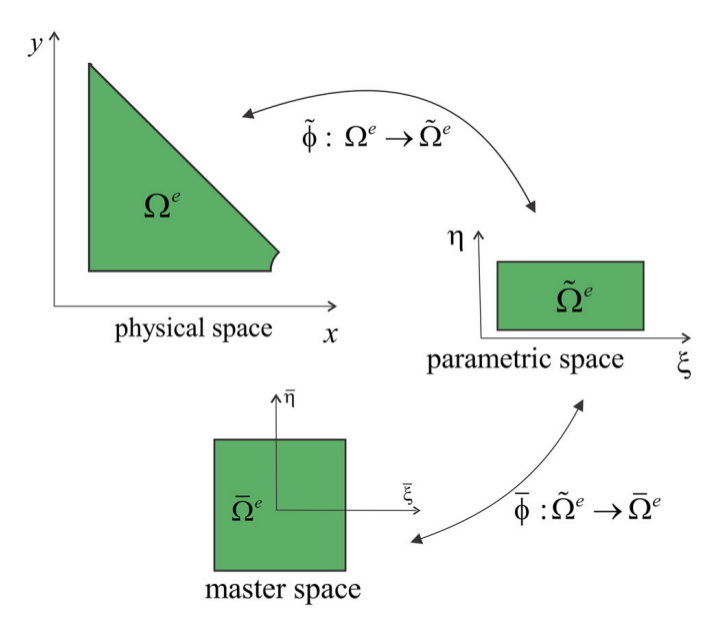
\includegraphics[scale=0.3]{Physical_Master.png} 
		\caption{\\Mapping IGA Physical element to Master element}\label{MasterPhysical}
	\end{center}	
\end{figure}


\begin{enumerate}[leftmargin=*]
	\item Mapping from master space to parametric space: \\
	Consider a discretized IGA surface which is defined in parametric space $\widetilde{\Omega_e}=[\xi_i,\xi_{i+1}]\otimes[\eta_i,\eta_{i+1}]$, Refer Fig.(). The NURBS basis functions and their derivatives are evaluated at $\xi,\eta$ of the element $\widetilde{\Omega_e}$. These $\xi,\eta$ co-ordinate values are calculated by a linear mapping as shown below
	\begin{equation}
	\xi=\frac{1}{2}[(\xi_{i+1}-\xi_{i})\overline{\xi}+(\xi_{i+1}+\xi_{i})]
	\end{equation} 
	\begin{equation}
	\eta=\frac{1}{2}[(\eta_{i+1}-\eta_{i})\overline{\eta}+(\eta_{i+1}+\eta_{i})]
	\end{equation}
	where $\overline{\xi},\overline{\eta}$ are the integration points defined in master space \\
	$\textbf{J}_2$ matrix is defined as 
	\begin{equation}
	\textbf{J}_2 = \frac{\partial\xi}{\partial \bar{\xi}} \frac{\partial\eta}{\partial \bar{\eta}}
	\end{equation} 
	Determinant of $\textbf{J}_2$ matrix is required in numerical integration scheme for linear mapping 
	
	
	\item Mapping from physical space to parametric space: \\
	The Jacobian matrix $\textbf{J}_1$ used to map from physical space to parametric space ($\Omega_e \rightarrow \widetilde{\Omega_e}$) is computed as:
	
	\begin{equation} \label{J1Matrix1}
	\textbf{J}_1 =
	\large
	\begin{bmatrix}
	\frac{\partial x}{\partial \xi} &\frac{\partial x}{\partial \eta} \\
	\frac{\partial y}{\partial \xi} &\frac{\partial y}{\partial \eta} \\
	\end{bmatrix} 
	\end{equation}
	
	The components of the $\textbf{J}_1$ matrix are calculated using Eq. (\ref{Co-ordinate}).
	
	\begin{equation}
	\frac{\partial x}{\partial \xi} = \sum_{k=1}^{n_{cp}^e} \frac{\partial \textbf{R}_k}{\partial \xi} x_i
	\qquad
	\frac{\partial x}{\partial \eta} = \sum_{k=1}^{n_{cp}^e} \frac{\partial \textbf{R}_k}{\partial \eta} x_i
	\end{equation} 
	
	\begin{equation}
	\frac{\partial y}{\partial \xi} = \sum_{k=1}^{n_{cp}^e} \frac{\partial \textbf{R}_k}{\partial \xi} y_i
	\qquad
	\frac{\partial y}{\partial \eta} = \sum_{k=1}^{n_{cp}^e} \frac{\partial \textbf{R}_k}{\partial \eta} y_i
	\end{equation}
	
\end{enumerate}
The two different mappings described above can be illustrated with an example considering $ \textbf{F}(x,y)$ integrated over the physical space $\Omega$

\begin{equation*}
\begin{split}
\int_{\Omega} \textbf{F}(x,y)d\Omega & = \sum_{e=1}^{nel} \int_{\Omega_e} \textbf{F}(x,y) d\Omega  \\
& = \sum_{e=1}^{nel} \int_{\widetilde{\Omega_e}} \textbf{F}(\xi,\eta)|\textbf{J}_1| d\xi d\eta \\
& = \sum_{e=1}^{nel} \int_{\overline{\Omega_e}} \textbf{F}(\overline\xi,\overline\eta)|\textbf{J}_1||\textbf{J}_2| d\overline\xi d\overline\eta  \\
& = \sum_{e=1}^{nel} \int_{-1}^{1} \int_{-1}^{1} \textbf{F}(\overline\xi,\overline\eta)|\textbf{J}_1||\textbf{J}_2| d\overline\xi d\overline\eta  \\
& = \sum_{e=1}^{nel} \left[ \sum_{i=1}^{n_{gp}^e} \textbf{F}(\overline\xi_i,\overline\eta_i) gw_i |\textbf{J}_1||\textbf{J}_2| d\overline\xi d\overline\eta \right]
\end{split}
\end{equation*}

\noindent
where $nel$ is the total number of elements and $n_{gp}^e$, $gw_i$ denotes the number of Gauss points and their respective Gauss weights.\\
\noindent
The formulated global stiffness matrix and force vector are solved using numerical scheme like Newton-Raphson method for the solution field.

\subsection{Post-processing Stage of the Analysis}
This section deals with visualization of the deformed geometry and how a displacement and stress fields are plotted. 

\begin{enumerate}[leftmargin=*]
	\item Visualization of the deformed NURBS geometry:
	
	Visualization of the deformed geometry will be done in the same manner as the visualization of the initial geometry. After determining the displacement field at control points they are added to the initial control points co-ordinates $[\textbf{P}]$.\\
	\\
	$[\textbf{P}_{new}]=[\textbf{P}]+[\textbf{U}]$ \\
	\\
	$[\textbf{P}^{new}]$ control points array is used to plot the deformed geometry.
	
	\item Plotting of displacement and stress fields:
	
	*** Have to write
\end{enumerate}

		\begin{figure}[H]
	\begin{center}
		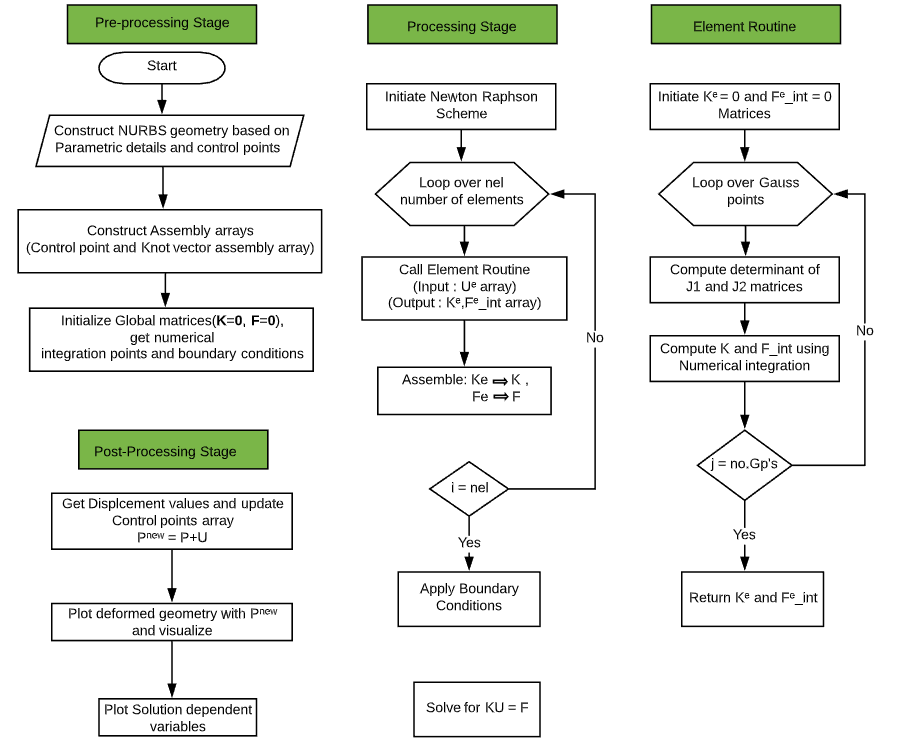
\includegraphics[scale=0.7]{FlowChart_cropped.png} 
		\caption{\\Flow chart describing Pre-processing, Processing and Post-processing Stage of IGA}\label{FlowChart1}
	\end{center}
	
\end{figure}


\section{Mechanical Case}


\subsection{Governing Equations}
The governing equation for mechanical deformation is based on conservation of linear momentum which can be written as
\begin{equation}
\sigma_{ij,i} + b_j = 0
\end{equation}
where $ \sigma_{ij} $ and $ b_i $ is the Cauchy stress tensor and body force. Due to the static nature of the analysis the inertial term is not included in the eq().\\*
Stress and strain are related by following constitutive equation
\begin{equation}
\sigma_{ij} = c_{ijkl} \epsilon_{kl}
\end{equation}
The infinitesimal strain theory is adopted for the analyis in which displacements of the material particles are considered to be very small compared to the dimentions of the body under loading. Strain in a small strain setting can be written as
\begin{equation}
\epsilon_{ij}=\frac{1}{2}[u_{i,j}+u_{j,i}]
\end{equation}
where $ u_{i} $ are the displacements in the body


\subsection{Weak Formulation}
Consider a domain $\Omega$ with $\Gamma_u$ as prescribed displacements and $\Gamma_t$ as traction boundary conditions. The domain boundary can be represented as $\Gamma = \Gamma_u \cup \Gamma_t$ and $\Gamma_u \cap \Gamma_t = \Phi$
By using the principle of virtual work the eq() can be written as
\begin{equation}
\delta W = \int_\Omega (\sigma_{ij,i} + b_j ) \delta u_j dV = 0
\end{equation} 
with,
$u = u_o$ on $\Gamma_u$ (essential boundary condition) and
$\sigma_{ij}n_j = \bar{t}_j$ on $\Gamma_t$ (natural boundary condition) \\*
where $\delta u_j$ is the virtual displacement field, $n_j$ is unit normal to the surface \\*
Applying integration by parts to the stress term under integral and by making using of conservation of angular momentum ($ \sigma_{ij} = \sigma_{ji} $) and Gauss divergence theorm (converting volume integral to surface integral) we approach at the following equation
\begin{equation} \label{FinalWeakform}
\delta W = \int_{\Omega} \sigma_{ij} \epsilon_{ij} d\Omega - \left[ \int_{\Gamma} \bar{t}_j \delta u_j d\Gamma_t  + \int_{\Omega} b_j \delta u_j d\Omega \right]
\end{equation}
as an additional requirement $\delta u_j$ must be zero at essential boundary conditions ($\Gamma_u$) for a unique solution.
***Additional data regarding detailed explanation of steps to derive weak form can be included.


\subsection{IGA Formulation}
The advantage of IGA over FEM formulation lies in its basis functions incorporation and its ability to capture the exact geometry. While the FEM uses lagrangian basis functions, IGA uses NURBS basis functions which are used to generate the geometry itself. As discussed in the previous sections a multidimentional NURBS basis function is represented by $R_{i,j,k}^{p,q,r}(\xi,\eta,\zeta) \rightarrow R_i$. The isogeometric element  is represented by basis function $R_i$ and control points $P_i$ as
\begin{equation} \label{Co-ordinate}
\textbf{x}^e = \sum_{i=1}^{n_{cp}^e} R_i P_i
\end{equation} 
By Galerkin approach, the displacements and virtual displacements are given by
\begin{equation} \label{u_and_du}
\textbf{u}^e = \sum_{i=1}^{n_{cp}^e} R_i \textbf{u}_i \qquad \delta\textbf{u}^e = \sum_{i=1}^{n_{cp}^e} R_i \delta\textbf{u}_i
\end{equation}
where $\textbf{u}_i$ and $\delta\textbf{u}_i$ are values at $i$th control point.
The strain displacement matrix \textbf{B} is given by
\begin{equation} \label{BMatrix}
\textbf{B} =
\begin{bmatrix}
R_{1,x} & 0 & 0 & R_{2,x} & 0 & 0 & .... & R_{n_{cp}^e,x} & 0 & 0 \\
0 &R_{1,y} & 0 & 0 & R_{2,y} & 0 & .... & 0 & R_{n_{cp}^e,y} & 0  \\
0 & 0 & R_{1,z} &0 & 0 & R_{2,z} & .... &0 & 0 & R_{n_{cp}^e,z}  \\
R_{1,y} & R_{1,x} & 0 & R_{2,y} & R_{2,x} & 0 & .... & R_{n_{cp}^e,y} & R_{n_{cp}^e,x} & 0 \\
0 & R_{1,z} & R_{1,y} & 0 & R_{2,z} & R_{2,y} & .... & 0 & R_{n_{cp}^e,z} & R_{n_{cp}^e,y}\\
R_{1,z} &0 & R_{1,x} & R_{2,z} &0 & R_{2,x} & .... &R_{n_{cp}^e,z} &0 &R_{n_{cp}^e,x}
\end{bmatrix}
\end{equation}
By substituting Eqs, (\ref{u_and_du}) and (\ref{BMatrix}) in Eq.(\ref{FinalWeakform}) the weak form in matrix terms can be written as
\begin{equation} \label{MatrixWeakForm}
\sum_{e=1}^{nel} \left[ \left( \int_{\Omega_e} \textbf{B}^T \textbf{C} \textbf{B} d\Omega \right) \right] \textbf{u} = \int_{\Gamma^e_t} \textbf{R}^T.\textbf{t} d\Gamma + \int_{\Omega^e_t} \textbf{R}^T.\textbf{f} d\Omega 
\end{equation}
where \text{R} is defined as \\
for the boundary $\Gamma^e$ 
\begin{equation} \label{RMatrix1}
\textbf{R} =
\begin{bmatrix}
R_1(\xi,\eta) & 0 & R_2(\xi,\eta) &0 & .... & R_{n_{cp}^e}(\xi,\eta) & 0 \\
0 &R_1(\xi,\eta) & 0 & R_2(\xi,\eta) & .... & 0 & R_{n_{cp}^e}(\xi,\eta) \\
\end{bmatrix}
\end{equation}
for the domain $\Omega^e$
\begin{equation} \label{RMatrix2}
\textbf{R} =
\begin{bmatrix}
R_1(\xi,\eta,\zeta) & 0 & R_2(\xi,\eta,\zeta) &0 & .... & R_{n_{cp}^e}(\xi,\eta,\zeta) & 0 \\
0 &R_1(\xi,\eta,\zeta) & 0 & R_2(\xi,\eta,\zeta) & .... & 0 & R_{n_{cp}^e}(\xi,\eta,\zeta) \\
\end{bmatrix}
\end{equation}
Eq.(\ref{MatrixWeakForm}) can be rewritten in a standard matrix form as
\begin{equation}
\sum_{e=1}^{nel} [\textbf{K}^e \textbf{U}^e = \textbf{F}^e] 
\end{equation}
where $\textbf{K}^e$ is isogeometric element’s stiffness matrix, $\textbf{U}^e$ is displacement vector and $\textbf{F}^e$ force vector





\section{Piezoelectric Case}


\subsection{Governing Equations for Piezoelectric Materials}
The coupled electro-mechanical interactions are governed by conservation of momentum and Gauss's law as:
\begin{equation} \label{MechEq}
\sigma_{ij,j} + f_i = 0
\end{equation} 
\begin{equation} \label{ElecEq}
D_{i,i} - q = 0
\end{equation}
Where, $ f_i $ is body force, $ q $ is electrical charge, $ \sigma_{ij} $ is Cauchy stress tensor and $ D_i $ is electrical displacement vector.
The constitutive equations for electromechanical coupling are defined as
\begin{equation}
\sigma_{ij} = C_{ijkl} \varepsilon_{kl} - e_{kij} E_k
\end{equation}
\begin{equation}
D_i = e_{ikl} \varepsilon_{kl} + \kappa_{ik} E_k
\end{equation}
Where, $ C_{ijkl} $ , $ e_{ikj} $ and $ \varepsilon_{ij} $ are elastic, piezoelectric and dielectric material constants respectively. The Cauchy stain tensor is defined as:
\begin{equation}
\varepsilon_{ij} = \frac{1}{2} (u_{i,j} + u_{j,i})
\end{equation}
and electric field vector as:
\begin{equation}
E_i = -\phi_{,i}
\end{equation}


\subsection{Weak Formulation}
Applying the principle of virtual work to the Eq.(\ref{MechEq})
and Eq. (\ref{ElecEq}) we can write
\begin{equation} \label{CouplingWeakForm1}
\int_\Omega ( \sigma_{ij,j} + f_i ) \delta u_i d\Omega = 0  
\end{equation}
\begin{equation} \label{CouplingWeakForm2}
\int_\Omega (D_{i,i} - q ) \delta \phi d\Omega = 0
\end{equation}
with, \\
essential boundary conditions:
$u = u_o$ on $\Gamma_u$ and $\Phi=\Phi_0$ on $\Gamma_\Phi$ \\
natural boundary condition:
$\sigma_{ij}n_j = \bar{t}_j$ on $\Gamma_t$ and $D_i n_i = q_0$ on $\Gamma_q$ \\*
where $\delta u_i$ and $\delta \phi$ are virtual or arbitrary displacement and potential fields. \\
Integrating Eq. (\ref{CouplingWeakForm1}) and Eq. (\ref{CouplingWeakForm2}) by parts and later applying Guass divergence theorm and boundary conditions we approach at weak form
\begin{equation} \label{FinalCouplingWeakForm1}
\int_\Omega \sigma_{ij} \delta \epsilon_{ij} d\Omega - \left[ \int_{\Gamma} \bar{t_i} \delta u_i d\Gamma + \int_\Omega f_i \delta u_i d\Omega  \right]= 0 
\end{equation}
\begin{equation} \label{FinalCouplingWeakForm2}
\int_\Omega D_i \delta E_i d\Omega - \left[ \int_{\Gamma} Q \delta \phi d\Gamma + \int_\Omega q \delta \phi d\Omega \right] = 0
\end{equation}


\subsection{IGA Formulation}
By Galerkin approach, displacements, potentials and their virtual values are given by below equations

\begin{equation} \label{u_and_du_2}
\textbf{u}^e = \sum_{i=1}^{n_{cp}^e} R_i \textbf{u}_i \qquad \delta\textbf{u}^e = \sum_{i=1}^{n_{cp}^e} R_i \delta\textbf{u}_i
\end{equation}

\begin{equation} \label{Phi_and_dPhi_2}
\Phi^e = \sum_{i=1}^{n_{cp}^e} R_i \Phi_i \qquad \delta\Phi^e = \sum_{i=1}^{n_{cp}^e} R_i \delta\Phi_i
\end{equation}

\noindent
where $\textbf{u}_i$ , $\delta\textbf{u}_i$, $\delta\Phi_i$ and $\Phi_i$ are values at $i$th control point.\\
By substituting Eqs, (\ref{u_and_du_2}) and (\ref{Phi_and_dPhi_2}) in Eq.(\ref{FinalCouplingWeakForm1}) and Eq.(\ref{FinalCouplingWeakForm2}) the weak form in matrix notation can be written as

\begin{equation} \label{CoupledStiffnessMatrix}
\begin{bmatrix} 
K_{MM} & K_{ME} \\
K_{EM} & K_{EE} \\ 
\end{bmatrix}
\begin{bmatrix} 
\textbf{u} \\
\phi \\ 
\end{bmatrix} = \begin{bmatrix} 
F_M \\
F_E \\ 
\end{bmatrix}
\end{equation}  
Where,
\begin{equation}
K_{MM} = \int_\Omega \textbf{B}_u^T \textbf{C} \textbf{B}_u d\Omega
\end{equation}
\begin{equation}
K_{ME} = \int_\Omega \textbf{B}_u^T \textbf{e} \textbf{B}_e d\Omega
\end{equation}
\begin{equation}
K_{EM} = \int_\Omega \textbf{B}_e^T \textbf{e}^T \textbf{B}_u d\Omega
\end{equation}
\begin{equation}
K_{EE} = - \int_\Omega \textbf{B}_e^T \kappa \textbf{B}_e d\Omega
\end{equation}
\begin{equation}
F_M = \int_\Omega \textbf{R}_u^T \textbf{f} d\Omega + \int_\Gamma \textbf{R}_u^T \textbf{t} d\Gamma 
\end{equation}
\begin{equation}
F_E = \int_\Omega \textbf{R}_e^T q d\Omega + \int_\Gamma \textbf{R}_e^T Q d\Gamma 
\end{equation}

\noindent
where \text{R} is defined as \\
for the boundary $\Gamma$ 

\begin{equation} \label{RMatrix1}
\textbf{R}_u =
\begin{bmatrix}
R_1(\xi,\eta) & 0 & R_2(\xi,\eta) &0 & .... & R_{n_{cp}^e}(\xi,\eta) & 0 \\
0 &R_1(\xi,\eta) & 0 & R_2(\xi,\eta) & .... & 0 & R_{n_{cp}^e}(\xi,\eta) \\
\end{bmatrix}
\end{equation}

\begin{equation} \label{RMatrix1}
\textbf{R}_e =
\begin{bmatrix}
R_1(\xi,\eta) & R_2(\xi,\eta) & .... & R_{n_{cp}^e}(\xi,\eta) \\
\end{bmatrix}
\end{equation}

\noindent
for the domain $\Omega$

\begin{equation} \label{RMatrix2}
\textbf{R}_u =
\begin{bmatrix}
R_1(\xi,\eta,\zeta) & 0 & R_2(\xi,\eta,\zeta) &0 & .... & R_{n_{cp}^e}(\xi,\eta,\zeta) & 0 \\
0 &R_1(\xi,\eta,\zeta) & 0 & R_2(\xi,\eta,\zeta) & .... & 0 & R_{n_{cp}^e}(\xi,\eta,\zeta) \\
\end{bmatrix}
\end{equation}

\begin{equation} \label{RMatrix2}
\textbf{R}_e =
\begin{bmatrix}
R_1(\xi,\eta,\zeta) & R_2(\xi,\eta,\zeta) & .... & R_{n_{cp}^e}(\xi,\eta,\zeta) \\
\end{bmatrix}
\end{equation}

\noindent
B matix is given as

\begin{equation} \label{BuMatrix}
\textbf{B}_u =
\begin{bmatrix}
R_{1,x} & 0 & 0 & R_{2,x} & 0 & 0 & .... & R_{n_{cp}^e,x} & 0 & 0 \\
0 &R_{1,y} & 0 & 0 & R_{2,y} & 0 & .... & 0 & R_{n_{cp}^e,y} & 0  \\
0 & 0 & R_{1,z} &0 & 0 & R_{2,z} & .... &0 & 0 & R_{n_{cp}^e,z}  \\
R_{1,y} & R_{1,x} & 0 & R_{2,y} & R_{2,x} & 0 & .... & R_{n_{cp}^e,y} & R_{n_{cp}^e,x} & 0 \\
0 & R_{1,z} & R_{1,y} & 0 & R_{2,z} & R_{2,y} & .... & 0 & R_{n_{cp}^e,z} & R_{n_{cp}^e,y}\\
R_{1,z} &0 & R_{1,x} & R_{2,z} &0 & R_{2,x} & .... &R_{n_{cp}^e,z} &0 &R_{n_{cp}^e,x}
\end{bmatrix}
\end{equation}

\begin{equation} \label{BeMatrix}
\textbf{B}_e =
\begin{bmatrix}
R_{1,x} & R_{2,x} & .... & R_{n_{cp}^e,x} \\
R_{1,y} & R_{2,y} & .... & R_{n_{cp}^e,y} \\
R_{1,z} & R_{2,z} & .... & R_{n_{cp}^e,z} \\
\end{bmatrix}
\end{equation}

\begin{equation}
\varepsilon = \textbf{B}_u . \textbf{u}
\end{equation}

\begin{equation}
\textbf{E} = - \textbf{B}_e . \Phi
\end{equation}

\noindent
Eq. (\ref{CoupledStiffnessMatrix}) can be solved using numerical methods like Newton Raphson scheme for displacements and potential solution field.

\section{Problem Description and Implementation}

\subsection{Problem statement}
A 2D piezoelectric plate subjected to mechanical displacements and electrical loading is considered as shown in Figure(\ref{2Dplate}) . The material used is PZT4 and material properties are as follows

$$
C = \begin{bmatrix}
139000 & 74280 & 77840 & 0 & 0 & 0\\
47280 & 115400 & 74280 & 0 & 0 & 0\\
77840 & 74280 & 139000 & 0 & 0 & 0\\
0 & 0 & 0 & 25640 & 0 & 0\\
0 & 0 & 0 & 0 & 25640 & 0\\
0 & 0 & 0 & 0 & 0 & 25640\\
\end{bmatrix} MPa
$$  
$$
e = \begin{bmatrix}
0 & -5.20710E-6 & 0 \\
0 & 15.08E-6 & 0 \\
0 & -5.207E-6 & 0\\
12.710E-6 & 0 & 0 \\
0 & 0 & 0 \\
0 & 0 & 12.710E-6 \\
\end{bmatrix} C/ mm`2
$$
$$
\varepsilon = \begin{bmatrix}
6.752E-12 & 0 & 0 \\
0 & 5.872E-12 & 0 \\
0 & 0 & 6.752E-12\\
\end{bmatrix} C/(V mm)
$$
where \\
C is Elastic constants, e is Piezoelectric constants and $\varepsilon$ being dielectric constants.

\begin{figure}[H]
	\begin{center}
	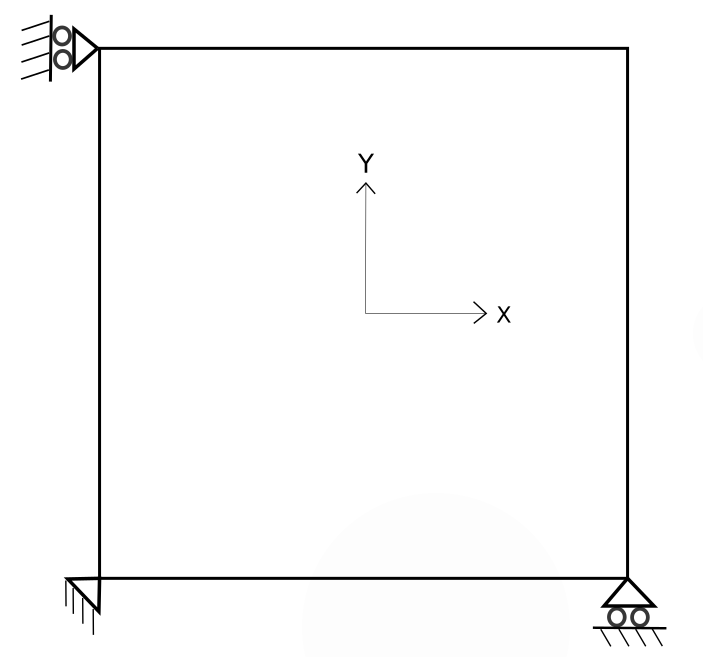
\includegraphics[scale=0.3]{2DPlate.png} 
	\caption{\\2D Piezoelectric plate}\label{2Dplate}
	\end{center}	
\end{figure}
\subsection{Parametric details for the plate with single element}
The 2nd order NURBS curve is used in both $\xi$ and $\eta$ directions. \\
\begin{comment}
The knot vectors along $\xi$ and $\eta$ directions are \\
$\Xi= [0,0,1,1]$ and $\eta= [0,0,1,1]$. \\
Control points along $\xi$ direction is given by \\
$n_{cp}(\xi)$ = total number of knots in $[\Xi] - (p+1) = 2$.\\
Similarly the total number of control points along $\eta$ direction is given by\\ $n_{cp}(\eta)$ = total number of knots in $[H ]- (q+1) = 2$ . \\
The total number of control points which defines the surface is\\
$n_{cp}$ = $n_{cp}(\xi) * n_{cp}(\eta)$ which is $2*2 = 4$. \\
\end{comment}
%\begin{verbatim}
\begin{enumerate}
\item Physical details for the geometry: \\
	L = 10 \qquad \# Length of the plate in mm \\
	H = 10 \qquad \# Height of the plate in mm \\

\item Parametric details of the geometry: \\
	U = [0,0,1,1] \#Knot vector in xi  direction \\
	V = [0,0,1,1] \#Knot vector in eta direction \\

    Degree of the curve \\
	p=1 \#Degree of the curve in xi  direction \\
	q=1 \#Degree of the curve in eta direction \\

	Number of control points in each direction \\
	ncpxi  = len(U) - (p+1)  \#No.of control points in xi  direction (4-(1+1) = 2) \\
	ncpeta = len(V) - (q+1)  \#No.of control points in eta direction (4-(1+1) = 2) \\

\item Total number of control points for the geometry \\
ncpxi*ncpeta = 2*2 = 4

#5. Control points for the geometry
P = [[[0,0,0,1],[L,0,0,1]],
[[0,L,0,1],[L,L,0,1]]]
\end{enumerate}
%\end{verbatim}
The control points are given by
\begin{center}
	\begin{tabular}{ |c|c|c|c|c| } 
		\hline
		i & $ P_{i,0} $ & $ P_{i,1} $  \\ \hline
		0 & $ (0,0,0,1) $ & $ (0,10,0,1) $  \\ \hline
		1 & $ (10,0,0,1) $ & $ (10,10,0,1) $  \\ \hline

	\end{tabular}
\end{center}
with fourth value in the paranthesis being weights of respective control points.
As this is the case of single element there is no need for the control point assembly array and knot vector connectivity matrix.









\noindent
%*** Remember References and citations ***
\bibliographystyle{plain}
\bibliography{References}
\end{document}
